\documentclass[10pt]{article}

\addtolength{\oddsidemargin}{-.875in}
\addtolength{\evensidemargin}{-.875in}
\addtolength{\textwidth}{1.75in}

\addtolength{\topmargin}{-.875in}
\addtolength{\textheight}{1.75in}

\openup 1em

%macro for commenting
\usepackage{color}
\newcommand{\leo}[1]{{\color{blue}{Leo: #1}}}

% \newcommand{\Xbeta}{ X_i \theta}
\newcommand{\xbeta}{ x_i \beta}
\newcommand{\xtheta}{ x_i \theta}
% \newcommand{\xbetaij}{ x_{ij}^T \theta}
\newcommand{\sgamma}{s_{ij}^T\gamma_i}

\usepackage[round]{natbib}

\usepackage{rotating}
\usepackage{graphicx}
\usepackage{subcaption}

\usepackage{float}
\usepackage{bbm}

\usepackage{amsthm,amsmath, amssymb} 
\usepackage{mathrsfs}
\usepackage{subcaption}
\usepackage{nicefrac}

\usepackage{xcolor}
\newcommand{\aki}[1]{\textcolor{red}{Aki: #1}}

\newtheorem{theorem}{Theorem}
\newtheorem{lemma}{Lemma}
\newtheorem{corollary}{Corollary}
\newtheorem{remark}{Remark}
\newtheorem{example}{Example}


\usepackage{algorithm}
\usepackage{algpseudocode}

%\usepackage{mhequ}
\newcommand{\be}{\begin{equation}\begin{aligned}}
\newcommand{\ee}{\end{aligned}\end{equation}}
\newcommand{\bb}[1]{\mathbb{#1}}
\newcommand{\mc}[1]{\mathcal{#1}}
\DeclareMathOperator{\Binom}{Binomial}
\DeclareMathOperator{\No}{No}
\DeclareMathOperator{\PG}{PG}
\DeclareMathOperator{\IG}{Inverse-Gamma}
\DeclareMathOperator{\Ga}{Gamma}
\DeclareMathOperator{\Bern}{Bernoulli}
\DeclareMathOperator{\U}{Uniform}
\DeclareMathOperator{\Poi}{Poisson}
\DeclareMathOperator{\NB}{NB}
\DeclareMathOperator{\cov}{cov}
\DeclareMathOperator{\var}{var}
\DeclareMathOperator{\diag}{diag}
\DeclareMathOperator{\Diag}{Diag}
\newcommand{\KL}[2]{\textnormal{KL}\left(#1 \parallel #2\right)}
\DeclareMathOperator{\1}{\mathbbm{1}}
\DeclareMathOperator{\bigO}{\mc O}
\newcommand{\dt}{\epsilon} % Stepsize of leapfrog
\newcommand{\mass}{M} % Mass matrix
\newcommand{\hess}{\mathbf{H}} % Hessian notation.



\thispagestyle{empty}
\baselineskip=28pt

\title{\textbf{Extrinsic Priors for Bayesian Modeling with Parameter Constraints}}
\author{Leo Duan, Akihiko Nishimura, David Dunson}
\date{}
\begin{document}
\maketitle
{\bf Abstract:} Prior information often takes for the form of parameter constraints. Bayesian methods include such information through prior distributions having constrained support. By using posterior sampling algorithms, one can quantify uncertainty without relying on asymptotic approximations. However, outside of narrow settings, parameter contraints make it difficult to develop efficient posterior sampling algorithms. We propose a general solution, which relaxes the constraint through the use of an {\em extrinsic prior}, which is concentrated close to the constrained space. General off the shelf posterior sampling algorithms, such as Hamiltonian Monte Carlo (HMC), can then be used directly. We illustrate this approach through multiple examples involving equality and inequality constraints. While existing methods tend to rely on conjugate families, our proposed approach frees us up to define new classes of hierarchical models for constrained problems. We illustrate this through application to a variety of simulated and real datasets.
\vskip 12pt
%\baselineskip=12pt
%\par\vfill\noindent
{\noindent KEY WORDS: Constraint relaxation; Euclidean Embedding; Monotone Dirichlet; Soft Constraint; Stiefel Manifold; Projected Markov chain}
%\par\medskip\noindent
%\clearpage\pagebreak\newpage
\pagenumbering{arabic}


\section{Introduction}
It is extremely common to have prior information available on parameter contraints in statistical models. For example, one may have prior knowledge that a vector of parameters lies on the probability simplex or satisfies a particular set of inequality constraints. Other common examples include shape constraints on functions, positive semidefiniteness of matrices and orthogonality. There is a very rich literature on optimization subject to parameter contraints. One common approach is to rely on Langrange and Karush-Kuhn-Tucker multipliers \citep{boyd2004convex}. However, simply producing a point estimate is often insufficient, as uncertainty quantification (UQ) is a key component of most statistical analyses. Usual large sample asymptotic theory, for example showing asymptotic normality of statistical estimators, tends to break down in constrained inference problems. Instead, limiting distributions may have a complex form that needs to be rederived for each new type of constraint, and may be intractable. An appealing alternative is to rely on Bayesian methods for UQ, including the constraint through a prior distribution having restricted support, and then applying Markov chain Monte Carlo (MCMC) to avoid the need for large sample approximations.

Conceptually MCMC can be applied in a broad class of constrained parameter problems without complications \citep{gelfand1992bayesian}. However, in practice, a primary difficulty is designing a Markov transition kernel that leads to an MCMC algorithm with sufficient computational efficiency to be practically useful. Common default transition kernels correspond to Gibbs sampling, random walk Metropolis-Hastings, and (more recently) Hamiltonian Monte Carlo (HMC). Gibbs sampling relies on alternately sampling from the full conditional posterior distributions for the different parameters, ideally in blocks to improve mixing. Gibbs requires the conditional distributions to be available in a form that is tractable to sample from directly, limiting consideration to specialized models. In constrained problems, block updating is typically either not possible or very inefficient (e.g. relying on rejection sampling with a high rejection probability), and one-at-a-time updating can lead to extremely slow mixing. Random walk algorithms provide an alternative, but each step of the random walk must maintain the parameter constraint. A common approach is to apply a normal random walk and simply reject proposals that violate the constraint, but this can have very high rejection rates even if using an adaptive approach that learns the covariance based on the history of the chain. An alternative is to rely on HMC. In simple settings in which a reparameterization can be applied to remove the constraint, HMC can be applied easily. Otherwise, HMC will generate proposals that violate the constraint, and hence face problems with high rejection rates in heavily constrained problems.

Due to the above hurdles, most of the focus in the literature has been on customized solutions developed for specific constraints.
One popular strategy is to carefully pick a prior and likelihood such that posterior sampling is tractable. For example, for modeling of data on manifolds, it is typical to restrict attention to specific models, such as the Bingham-von Mises-Fisher distribution for Stiefel manifolds \citep{khatri1977mises,hoff2009simulation}. For data on the probability simplex, one instead relies on the Dirichlet distribution. An alternative is to reparameterize the model to eliminate or simplify the constraint. For example, when faced with a monotonicity constraint, one may reparameterize in terms of differences as the resulting positivity constraint leads to much easier sampling \citep{dunson2003bayesian,gunn2005transformation}. In the literature on modeling of data on manifolds, there are two strategies: (i) {\em intrinsic} methods that define a statistical model directly on the manifold, and (ii) {\em extrinsic} methods that indirectly induce a model on the manifold through embedding the manifold in a Euclidean space, defining a model in the Euclidean space, and then projecting back onto the manifold. Essentially all of the current strategies for Bayesian modeling with constraints take an intrinsic-style approach. However, by strictly maintaining the constraint at all stages of the modeling and computation process, one limits the possibilities in terms of defining general methods to deal with parameter constraints.

These drawbacks motivate the development of {\em extrinsic} approaches that define an unconstrained model and/or computational algorithm, and then somehow adjust for the constraint. A related idea is \cite{gelfand1992bayesian}, who suggested running Gibbs sampling ignoring the constraint but only accepting the draws satisfying the constraint. Unfortunately, such an approach is highly inefficient, as motivated above. An alternative is to run MCMC ignoring the constraint, and then project draws from the unconstrained posterior to the appropriately constrained space. Such an approach was proposed for generalized linear models with order constraints by \cite{dunson2003bayesian}, extended to functional data with monotone or unimodal constraints \cite{gunn2005transformation}, and recently modified to nonparametric regression with monotonicity \cite{lin2014monogp} or manifold \cite{lin2016extrinsic} constraints.

An alternative idea is to {\em relax} a sharp parameter constraint by defining a prior that has unrestricted support but places small probability outside of the constrained region. \cite{neal2011mcmc} suggested such an approach to apply HMC in settings involving a simple truncation constraint, while \cite{pakman2014exact} applied a related idea to improve sampling from truncated multivariate normal distributions.

The goal of this article is to dramatically generalize these specific approaches to develop a broad class of {\em extrinsic priors} for parameter constrained problems. These priors are defined to place small probability outside of the constrained region, while permitting use of efficient and general use MCMC algorithms; in particular, HMC. Unlike intrinsic methods, such as Riemannian and geodesic HMC \citep{girolami2011riemann,byrne2013geodesic}, our approach is simple to implement in general settings using automatic algorithms. The generality frees up a much broader spectrum of Bayesian models, as one no longer needs to focus on very specific computationally tractable models.
Theoretic studies are conducted and original models are shown in simulations and data applications.

\section{Extrinsic Bayes Methodology}

\subsection{Conditional Intrinsic Distribution}

Let $\theta \in \mc D$ denote the parameters in likelihood function $L(\theta;y)$, with $y$ the data. The support $\mc D$ is a constrained space. The usual Bayesian approach assigns a prior density $\pi_{0,\mc D}(\theta)$ for $\theta$ having support $\mc D$. 
A common strategy is to reparameterize $\theta$ with $f(\theta)$ to always satisfy $\theta \in \mc D$, and find an {\it intrinsic} distribution on $\mc D$, such as the famous stick-breaking construction for probability simplex. Although this strategy is successful, reparameterization does not always exist.

We now first present a much more general construction by inducing a {\it conditional} intrinsic distribution. Starting from a prior $\pi_{0,\mc R}(\theta)$ on a `less constrained' space $\mc R\supset \mc D$, we constrain it on $\mc D$ by inducing its conditional density given $\theta\in \mc D$. For simplicity, we focus on $\mc R$ being Eucledean space $\mathbb{R}^{p}$ or its truncated subspace. Letting  $v: \bb{R}^p\rightarrow \bb [0,\infty)^d$ Lipschitz with $p>d$ define a measurable distance to the constrained space $\mc D$, then constrained space is associated with $\mc D = \{\theta\in \mc R:v(\theta)=\bf 0\}$. The conditional probability of $\theta\in B$ given $\theta\in D$ is:

\begin{equation}
\label{intrinsicPrior}
	\int_{B}\pi_{0,\mc D}(\theta)d\theta= \frac{1}{m(\bf 0)}\int_{B} \frac{\pi_{0,\mc R}(\theta) \mathbbm{1}_{v({\theta})={\bf 0}}}{J_p v(\theta)}\mc H^{p-d}(d\theta)
\end{equation}
if $0<m(\bf 0)<\infty$, else $\int_{B}\pi_{0,\mc D}(\theta)d\theta= \delta_{x^*}(B)$, a point mass at some fixed $x^{*}\in \bb R^p$; $m(x)= \int \frac{\pi_{0,\mc R}(\theta)\mathbbm{1}_{v({\theta})=x}}{J_p v(\theta)}\mc H^{p-d}(d\theta)$ is the marginal density of $v$; $\mc H^{k}(d\theta)$ is a $k$-dimensional Hausdorff measure and equal to $\frac{\Gamma(\frac{k}{2}+1)}{\Gamma(\frac{1}{2})^k} d\theta$ when $k$ is an integer;  $J_p v(\theta) = \sqrt{\det (D\theta' D\theta)}$  with $D\theta$ as the derivative matrix if $\det (D\theta' D\theta)>0$, or $J_p v(\theta) =1$ if $\det (D\theta' D\theta)=0$. It is shown that \eqref{intrinsicPrior} is a valid regular conditional probability \citep{diaconis2013manifold}.

Given data $y$, the posterior probability of set $B$ is
\begin{equation}
\label{intrinsicPosterior}
	\int_{B}\pi_{\mc D}(\theta \mid y)d\theta= \frac{1}{m({\bf 0} \mid y)}\int_{B} \frac{L(\theta;y)\pi_{0,\mc R}(\theta) \mathbbm{1}_{v({\theta})={\bf 0}}}{J_p v(\theta)}\mc H^{p-d}(d\theta)
\end{equation}
if $0<m({\bf 0} \mid y)<\infty$, else $\int_{B}\pi_{\mc D}(\theta \mid y)d\theta= \delta_{x^*}(B)$, a point mass at some fixed $x^{*}\in \bb R^p$; $m(x\mid y)= \int \frac{L(\theta;y)\pi_{0,\mc R}(\theta)\mathbbm{1}_{v({\theta})=x}}{J_p v(\theta)}\mc H^{p-d}(d\theta)$ is the marginal density of $v$ given $y$.

In general, \eqref{intrinsicPrior} and \eqref{intrinsicPosterior} are analytically intractable and difficult to approximate with Monte Carlo sampling, due to the indicator function $\mathbbm{1}_{v({\theta})={\bf 0}}$ that constrains $\theta\in \mc D$; although closed-form may exist for some simple case. To illustrate, we use one toy example throughout this section.

{\bf Example 1A: Two Gaussians with Sum Constraint (Conditional Intrinsic Approach)}

Consider a bivariate Gaussian random vector $[\theta_1,\theta_2]' \sim \No(0,I)$ in constrained space $\mc D=\{(\theta_1,\theta_2):\theta_1+\theta_2-1=0\}$. Denoting $\phi(x)= \frac{1}{\sqrt{2\pi}} \exp(-\frac{x^2}{2})$, for set $B= \{(\theta_1,\theta_2): \theta_1< x, \theta_2\in \mathbb R\}$, $J_2v(\theta)=2$.

\begin{equation*}
	\begin{aligned}
\int_{B} \pi_{0,\mc D}(\theta) d\theta= 
& \frac{
\int_{-\infty}^{x} \frac{1}{2}\phi(\theta_1)\phi(\theta_2)\mathbbm{1}_{\theta_1+\theta_2-1=0} \frac{\Gamma(\frac{1}{2}+1)}{\Gamma(\frac{1}{2})}  d\theta_1  
}{\int_{-\infty}^{\infty}\frac{1}{2}\phi(\theta_1)\phi(\theta_2) \mathbbm{1}_{\theta_1+\theta_2-1=0}  \frac{\Gamma(\frac{1}{2}+1)}{\Gamma(\frac{1}{2})}   d\theta_1} \\ 
=& \frac{
\int_{-\infty}^{x}\frac{1}{2}\phi(\theta_1)\phi(1-\theta_1)d\theta_1  
}{
\int_{-\infty}^{\infty}\frac{1}{2}\phi(\theta_1)\phi(1-\theta_1)d\theta_1  } \\ 
= & \int_{-\infty}^{x} \frac{\sqrt{2}}{\sqrt{2\pi}} \exp(-\frac{(\theta_1-\frac{1}{2})^2}{2/2}) d\theta_1,
\end{aligned}
\end{equation*}
which corresponds to $\theta_1\mid (\theta_1+ \theta_2=1) \sim \No(1/2,1/2)$, $\theta_2\mid \theta_1 \sim \delta_{1-\theta_1}(.)$. Marginally, this is a degenerate bivariate Gaussian distribution:
$$\begin{bmatrix} \theta_1 \\ \theta_2 \end{bmatrix} \sim
\No_{\text d} \left(
 \begin{bmatrix} \frac{1}{2} \\ \frac{1}{2} \end{bmatrix},
\begin{bmatrix} \frac{1}{2} & -\frac{1}{2}  \\  -\frac{1}{2}  & \frac{1}{2} \end{bmatrix}
\right).$$



\subsection{Extrinsic Bayes}
We now propose an extrinsic distribution that builds on \eqref{intrinsicPrior} and \eqref{intrinsicPosterior}, approximating the sharp $\mathbbm{1}_{v(\theta)= \bf 0}$ with a {\em smooth} alternative $\mc{K}( \theta; \mc D)$ with less contrained support:


\begin{equation}
\label{extrinsicPrior}
	\int_{B}\tilde \pi_{0,\mc D}(\theta)d\theta= \frac{1}{m}\int_{B} \frac{\pi_{0,\mc R}(\theta) \mc{K}( \theta; \mc D)   }{J_p v(\theta)}\mc H^{p-d}(d\theta)
\end{equation}
where $m=\int_{\mc R} \frac{\pi_{0,\mc R}(\theta) \mc{K}( \theta; \mc D)   }{J_p v(\theta)}\mc H^{p-d}(d\theta)$. The posterior takes similar form
\begin{equation}
\label{extrinsicPosterior}
	\int_{B}\tilde \pi_{\mc D}(\theta \mid y)d\theta= \frac{1}{m}\int_{B} \frac{L(\theta;y)\pi_{0,\mc R}(\theta) \mc{K}( \theta; \mc D)   }{J_p v(\theta)}\mc H^{p-d}(d\theta)
\end{equation}
with $m=	\int_{\mc R} \frac{L(\theta;y)\pi_{0,\mc R}(\theta) \mc{K}( \theta; \mc D)   }{J_p v(\theta)}\mc H^{p-d}(d\theta)$.
 
The function $\mc K(\theta;\mc D)$ maps from $\bb R^p\rightarrow [0,1]$ and is defined as:

\begin{equation}
\label{smoothing}
\mc K(\theta; \mc D)= \prod_{k=1}^d K_k(v_k(\theta)),
\end{equation}
where $v_k(\theta)$ corresponds to left hand side of the $k$th equation in $v(\theta)=\bf 0$, as defined in the last section. Instead of assigning point mass at $v(\theta)=\bf 0$, $K_k$ assigns mass {\it concentrated} at $0$ with low but positive density for ${v_k(\theta)>0}$. This expands the sampling space from $\mc D$ to $\mc R$. For simplicity, from now on we focus on exponential smoothing function $K_k(v(\theta))=\exp(-\frac{v(\theta)}{\lambda_k})$ with $\lambda_k>0$ as a tuning parameter.

We now elaborate the notion of distance $v_k(\theta)$. Assuming there are $d$ constraints with each defining a constrained subspace $\mc D_k$, $\mc D = \bigcap_{k=1}^d\mc D_k$, then $v_k: \mc R \rightarrow [0,\infty)$ is a measurable function and quantifies the distance to space $\mc D_k$. For $k=1,\ldots,m$, $v_k(\theta)=0$ only if $\theta\in \mc D_k$. For example, one can use $v(\theta)=|f(\theta)|$ as a distance to equality-constrained space  $\{\theta:f(\theta)=0\}$; $v(\theta)=|f(\theta)|_+$, where $(x)_+ = \left\{\begin{array}{cc}  0 \text{ if } x\le 0 \\ x \text{ if } x> 0\end{array}\right.$ as a distance to inequality-constrained space  $\{\theta:f(\theta) \le 0\}$. This idea is flexible to accomodate more complicated scenarios. For example, $\theta$ can have only a subset of parameters constrained; parameters can be in multiple constraints simultaneously; constraints can be dependent. 

To summarize, $\theta\in \mc D$ $\Leftrightarrow$ all $v_k(\theta)=0$ $\Leftrightarrow$ $\mc K(\theta; \mc D)=1$, leading to $\mc K(\theta; \mc D)=\mathbbm{1}_{\theta\in \mc D}$ if $\theta\in \mc D$, but $\mc K(\theta; \mc D)>0$ if  $\theta\not\in \mc D$. To provide some intuition about the smoothing, Figure~\ref{truncated_normal} plots the densities of a truncated normal prior $\No_{(-\infty,5)}(0,5^2)$ and the extrinsic approximation. We use $\mc K(\theta;\mc D)=\exp(-v(\theta))$ with $v(\theta)=(\theta-5)_+$ and $v(\theta)=(\theta-5)^2_+$ as two example distances. Inside $\mc D=(-\infty,5)$, both intrinsic and extrinsic distribution are the same, except for a different normalizing constant; outside $\mc D$, intrinsic one drops directly to $0$ at the boundary, whereas the extrinsic one decreases smoothly.

\begin{figure}[H]
 \centering
 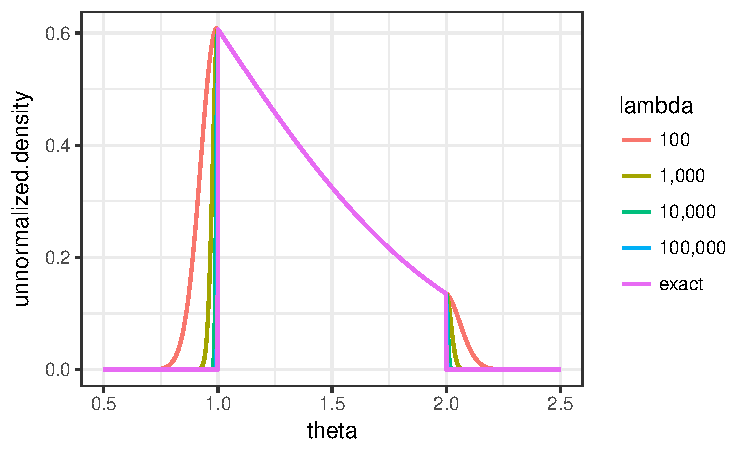
\includegraphics[width=0.5\textwidth]{density_truncated_normal}
\caption{Unnormalized densities for truncated normal $\No_{(-\infty,5)}(0,5^2)$ under exact intrinsic prior and approximating extrinsic prior. Inside $(-\infty,5)$, the priors are the same up to a constant difference. The intrinsic prior abruptly drops to $0$ on the boundary, while the approximating ones drop smoothly. Intrinsic prior based on first-order $v(\theta)$ drops faster than the one based on second order when $v(\theta)\in (0,1)$.}
\label{truncated_normal}
\end{figure}

We now return to the previous example of two Gaussians under sum constraint, applying extrinsic Bayes technique.

{\bf Example 1B: Two Gaussians with Sum Constraint (Extrinsic Approach)}

We use extrinsic prior $\tilde\pi_{0,\mc D}(\theta) \propto \exp(-\frac{\theta_1^2+\theta_2^2}{2})\exp(-\frac{v(\theta)}{\lambda})$. Choosing $v(\theta)= (\theta_1+\theta_2-1)^2$ allows us to obtain closed-form for the extrinsic prior $\theta_1 \sim \No(\frac{2}{\lambda+4},\frac{\lambda+2}{\lambda+4})$, $\theta_2\mid \theta_1 \sim \No(\frac{2}{\lambda+2}(1-\theta_1),\frac{\lambda}{\lambda+2})$. Marginally, 

$$\begin{bmatrix} \theta_1 \\ \theta_2 \end{bmatrix} \sim
\No \left(
 \begin{bmatrix} \frac{2}{\lambda+4} \\ \frac{2}{\lambda+4} \end{bmatrix},
\begin{bmatrix} \frac{\lambda+2}{\lambda+4} & -\frac{2}{\lambda+4}  \\  -\frac{2}{\lambda+4}  &\frac{\lambda+2}{\lambda+4} \end{bmatrix}
\right).$$
As $\lambda\rightarrow 0$, the extrinsic prior becomes the same as the degenerate bivariate Gaussian in intrinsic approach.

For more general cases, \eqref{extrinsicPrior} and \eqref{extrinsicPosterior} do not have closed-form; however, it is now easy to use conventional Monte Carlo techniques since $\mc K(\theta;\mc D)$ expands the space from $\mc D$ to $\mc R$.

\subsection{Approximation Error}
We now quantify approximation error of extrinsic distribution. Due to similar form in prior and posterior, we now introduce some general notation. Let $\pi_{\mc R}(\theta)$ be the normalized density in $\mc R$ such that $\int \pi_{\mc R}(\theta)=1$, which is $\pi_{0,\mc R}(\theta)$ for prior and $L(y;\theta)\pi_{0,\mc R}(\theta)$ for posterior; $\Pi(.)$ and $\tilde\Pi(.)$ to represent the measures under intrinsic and extrisic distributions. 

Suppose $\Phi:\mathbb R^p \rightarrow \mathbb R^d$ with $p>d$ is Lipschitz, then the co-area formula \citep{federer2014geometric} is,
	\begin{equation}
\ \int_{\mathbb{R}^n}  f(\theta)J_N\Phi(\theta)\mu^n(d \theta)
	=\ \int_{\mathbb{R}^m}  \int_{\Phi^{-1}(y)}f(\theta) \mc H^{n-m}(d\theta)\mu^m(d y),
	\end{equation}
where $\mu^k(d\theta)$ a $k$-dimensional Lebesgue measure. We first re-parameterize $\mc K(\theta;\theta)$ as $\exp(-\lambda^{-1}  v(\theta))$ where $\lambda=\max_k \lambda_k$ and $v(\theta)=\prod_{k=1}^d\frac{v_k(\theta)}{\lambda^*_k}$ with $\lambda^*_k=\lambda_k/\lambda$. Having $\Phi(\theta)=v(\theta)$ yields $J v(\theta)=\|\nabla v(\theta)\|$ if $\|\nabla v(\theta)\|>0$ and $J v(\theta)=1$ if $\|\nabla v(\theta)\|=0$.

Having $f(\theta)=\frac{\pi_{\mc R}(\theta)}{J v(\theta)}$ and $f(\theta)=\frac{\pi_{\mc R}(\theta)g(\theta)}{J v(\theta)}$ yield the marginal density and conditional expectation, respectively:
\begin{equation}
	\begin{aligned}
m(x)= & \int_{v^{-1}(x)} \frac{ \pi_{\mc R}(\theta) }{ J v(\theta) } \mathcal{H}^{p-d}(d \theta),\\
\mathbb{E}(g(\theta) \mid x)= & \int_{v^{-1}(x)} \frac{ g(\theta) \pi_{\mc R}(\theta)}{ J v(\theta) } \mathcal{H}^{p-d}(d \theta).
		\end{aligned}
\end{equation}

Comparing the posterior samples from intrinsic and extrinsic distributions, the 1-Wasserstein distance $W_1(\Pi,\tilde\Pi)$ represents the minimal amount of transport needed to transform one distribution to another. Formally, it is defined as

$$W_1(\Pi,\tilde\Pi)=\underset{\gamma\in \Gamma(\Pi,\tilde\Pi)}{\inf}\int \|x-y\| d\gamma(x,y)$$ 
where $\Gamma(\Pi,\tilde\Pi)$ is the family of all joint measures of the two samples with $\Pi$ and $\tilde\Pi$ as the marginals.

\begin{remark}
The 1-Wasserstein distance between the extrinsic and intrinsic distributions has
$$ \underset{\lambda \rightarrow 0}\lim W_1(\Pi,\tilde\Pi)=0.$$
Further,  letting $k_1=\underset{g:\|g\|_L\le 1}\sup\underset{t^*\in [0,t)}\sup \|\mathbb{E}(g(\theta) \mid t^*)\|$, $k_2=\underset{g:\|g\|_L\le 1} \sup \mathbb{E}(\| g(\theta )\|)$, $k_3= \underset{t^*\in (0,t)}\sup  m(t^{*})$,

\begin{equation}
\begin{aligned}
W_1(\Pi,\tilde\Pi) \le \lambda (\frac{k_1 k_3}{m_0^2} + \frac{k_1}{m_0}) + \exp(- \lambda^{-1} t )(\frac{k_1}{m_0^2} + \frac{k_2}{m_0}),
\end{aligned}
\end{equation}
if there exists a $t$-ball surrounding $\mc D$, $\{\theta: v(\theta)<t\}$ having bounded marginal density for $v(\theta)$ and conditional expectation for any Lipschitz functions, $k_1,k_3= \mc O(1)$ and the expectation over $\mc R$ has $k_2 = \mc O(\lambda \exp(\lambda^{-1} t))$, $W_1(\Pi,\tilde\Pi)$ converges to $0$ in $\mc O(\lambda)$.


\end{remark}

The proof is provided in the appendix.


\section{Posterior Computation}

One particular appeal of the extrinsic approach is its advantage in posterior computation. As it is supported on a less restrictive space $\mc R$, one can exploit conventional sampling tools such as slice sampling, adaptive Metropolis-Hastings and Hamiltonian Monte Carlo (HMC). In this section, we focus on HMC for its easiness to use and good performance in sampling with high-dimensional parameters.

\subsection{Hamiltonian Monte Carlo for Extrinsic Posterior Sampling}

We provide a brief overview of HMC for continuous $\theta$ under extrinsic prior. Discrete extension is possible via recent work of \cite{nishimura2017discontinuous}.

In order to sample from $\theta\in\mc R \subset \mathbb R^d$, HMC introduces an auxillary momentum variable $p \sim \No(0, \mass)$. The covariance matrix $\mass$ is referred to as a \textit{mass matrix} and is typically chosen to be the identity or adapted to approximate the inverse covariance of $\theta$. HMC then sample from the joint target density $\pi(\theta, p) = \pi(\theta) \pi(p) \propto \exp (- H(\theta, p))$ where, in the case of an extrinsic posterior \eqref{extrinsicPosterior}, 


\begin{equation}
\begin{aligned}
H(\theta, p)& = U(\theta)+K(p),\\
\text{where } & U(\theta) = -\log\left\{ L(\theta;y)\pi_{0,\mc R}(\theta) \mc{K}(\theta;\mc D) / J(v(\theta)) \right\},\\
& K(p) = \frac{p'\mass^{-1} p}{2}.
\end{aligned}
\end{equation}

From the current state $(\theta^{(0)},p^{(0)})$, HMC generates a proposal for Metropolis-Hastings algorithm by simulating Hamiltonian dynamics, which is defined by a differential equation:

\begin{equation}
\begin{aligned}
\label{hamiltonian}
\frac{\partial \theta ^{(t)}}{\partial t} & =\frac{\partial H(\theta, p)}{\partial p} = \mass^{-1}p,\\
\frac{\partial p^{(t)}}{\partial t}& =-\frac{\partial H(\theta, p)}{\partial \theta} = -\frac{\partial U(\theta)}{\partial \theta}.
\end{aligned}
\end{equation}

The exact solution to \eqref{hamiltonian} is typically intractable but a valid Metropolis proposal can be generated by numerically approximating \eqref{hamiltonian} with a reversible and volume-preserving  integrator \citep{neal2011mcmc}. The standard choice is the \textit{leapfrog} integrator which approximates the evolution $(\theta^{(t)},p^{(t)}) \to (\theta^{(t + \dt)},p^{(t + \dt)})$ through the following update equations:

\begin{equation}
\begin{aligned}
\label{leap-frog}
p \leftarrow p - \frac{\dt}{2} \frac{\partial U}{\partial  \theta },\quad
\theta \leftarrow  \theta  + \dt \mass^{-1}p,\quad
p \leftarrow p -  \frac{\dt}{2}  \frac{\partial U}{\partial  \theta } 
\end{aligned}
\end{equation}
Taking $L$ leapfrog steps from the current state $(\theta^{(0)},p^{(0)})$ generates a proposal $(\theta^{*},p^{*}) \approx (\theta^{(L \dt)},p^{(L \dt)})$, which is accepted with the probability 
$$1\wedge \exp  \left( - H(\theta^{*},p^{*}) + H(\theta^{(0)},p^{(0)}))\right)$$


\subsection{Support Expansion and Computing Efficiency}

While an extrinsic distribution more closely approximate the constraint with a smaller $\lambda$, computational efficiency of HMC can be negatively impacted by choosing $\lambda$ too small in certain condition. In this section, we explain and quantify this phenomenon and provide a practical guidance on how to pick a reasonable value of $\lambda$.

In understanding the computational efficiency of HMC, it is useful to consider the number of leapfrog steps to be a function of $\dt$ and set $L = \lfloor \tau / \dt \rfloor$ for a fixed \textit{integration time} $\tau > 0$. In this case, the mixing rate of HMC is completely determined by $\tau$ in the limit $\dt \to 0$ \citep{betancourt17}. In practice, while a smaller stepsize $\dt$ leads to a more accurate numerical approximation of Hamiltonian dynamics and hence a higher acceptance rate, it takes a larger number of leapfrog steps and gradient evaluations to achieve good mixing. For an optimal computational efficiency of HMC, therefore, the stepsize $\dt$ should be chosen only as small as needed to achieve a reasonable acceptance rate \citep{beskos13, betancourt14}. A critical factor in determining a reasonable stepsize is the \textit{stability limit} of the leapfrog integrator \citep{neal2011mcmc}. When $\dt$ exceeds this limit, the approximation becomes unstable and the acceptance rate drops dramatically. Below the stability limit, the acceptance rate $a(\dt)$ of HMC increases to 1 quite rapidly as $\dt \to 0$ and in fact satisfies $a(\dt) = 1 - \mc O(\dt^4)$ \citep{beskos13}.

For simplicity, the following discussions assume the mass matrix $\mass$ is taken to be the identity. Let $\hess_U(\theta)$ denote the hessian matrix of $U(\theta) = - \log \pi(\theta)$ and let $\omega_1(\theta)$ denotes the first largest eigenvalue of $\hess_U(\theta)$. While analyzing stability and accuracy of an integrator is highly problem specific, the linear stability analysis and empirical evidences suggest that, for stable approximation of Hamiltonian dynamics by the leapfrog integrator in $\bb R^p$, the condition $\dt < 2\omega_1(\theta)^{-1/2}$ must hold on most regions of the parameter space $\theta$ \citep{hairer06}.
When $\theta$ is strictly constrained in certain region, $\theta\in \mc D^*_1$, another limiting factor is the shortest distance to the boundary $\eta (\theta; {\mc D^*_1})= \inf_{\theta^*\not\in D_1^*}\|\theta^*-\theta\|$. Therefore,

\begin{equation}
\label{stabilityCondition}
\dt <  \eta (\theta; {\mc D^*_1}) \wedge 2\omega_1(\theta)^{-1/2} 
\end{equation}

In the case of an extrinsic posterior with $\mc K(\theta;\mc D)= \prod_{k=1}^{d} \exp(- \lambda_k^{-1}v_k(\theta))$, the Hessian $\hess_U(\theta)$ is given by
\begin{equation}
\label{eq:hessian_extrinsic}
\hess_U(\theta) = -\hess_{\log \pi_\mc R}(\theta)+\sum_k \lambda_k^{-1} \hess_{v_k}(\theta) \mathbbm{1}_{\theta\not\in \mc D_k},
\end{equation}
where in the first term $\pi_\mc R(\theta)=\pi_{0,\mc R}(\theta)L(\theta;y)/Jv(\theta)$ is defined on all $\mc R$, while in the second term $\lambda_k^{-1} \hess_{v_k}(\theta) \mathbbm{1}_{\theta\not\in \mc D_k}$ is $0$ unless $\theta\not\in \mc D_k$.  When $\theta\not\in \mc D_k$, the eigenvalue of \eqref{eq:hessian_extrinsic} is commonly dominated by $\lambda^{-1}_k$.

The key for computational efficiency is to prevent the bound in \eqref{stabilityCondition} from being too close to $0$. This can be achieved by strictly upholding certain constraints while relaxing more constrigent ones. Formally, recall $\mc D=\cap_{k=1}^d \mc D_k$, $\{\mc D_k\}$ can be into two sets, $\{\mc D_{(1)}, \mc D_{(2)}, \ldots , \mc D_{(m)} \}$ and $\{\mc D_{(m+1)}, \mc D_{(m+2)}, \ldots , \mc D_{(d)} \}$, such that  for most region in $\mc D^*_1= \cap_{j=1}^m \mc D_{(j)}$, $\eta(\theta;{\mc D^*_1})$ is away from $0$, but $\mc D^*_1 \cap D_{(j')}$ for any $j'= m+1, \ldots, d$ has $\eta(\theta; \mc D^*_1 \cap D_{(j')})\approx 0$. As $\lambda_{(j)}$ controls the amount of relaxation, one can use $\lambda_{(j)}\approx 0$ for $j=1,\ldots,m$ to force $\theta \in \mc D_1^*$ for most of the time, while moderately small $\lambda_{(j')}$ for $j'=(m+1),\ldots,d$ to allow $\theta\not \in \mc D_{(j')}$ to happen. As the result, the effective stability bound is:


\begin{equation}
\label{optimalStabilityCondition}
\dt <  \eta(\theta;{\cap_{j=1}^m \mc D_{(j)}})  \wedge \left(2 \min_{j'\in \{m+1,\ldots,d\}}\lambda_{(j')}^{1/2}\right)
\end{equation}
Generally, often one can use very small $\lambda_j$ to almost perfectly uphold inequality constraints, as they do not lead to small $\eta(.)$ in the first term; whereas equality constraints need relaxation with moderate $\lambda_{j'}$ in the second term, as they commonly define hyper-plane that has $\eta(.)\approx 0$.

For $\lambda_{j'}$ not very close to $0$, a trade-off between approximation accuracy and computational efficiency is involved. Fortunately,  the approximation error $\mc O( \underset{j'\in \{m+1,\ldots,d\}} \max\lambda_{(j')})$ decreases faster than the efficiceny cap $\mc O( \underset{j'\in \{m+1,\ldots,d\}} \min\lambda^{1/2}_{(j')})$. For example, empirically we found $\lambda_{j'}=10^{-4}$ often yields a very low approximation error; reducing the error tolerance $10$ times 
lower only requires approximately $3$ times of computing budget.


\section{Simulated Examples and Application}

We now use examples to illustrate the properties of extrisinc priors and their utility in common scenarios.

\subsection{Simulations}

We first use two examples to demonstrate how to choose $\lambda_{k}$'s, depending on the geometry of $\mc D$.

{\bf Example 2: Linear Regression Under Linear Inequality}

Consider a linearly constrained regression model:

$$y_i \sim \No (x_i \theta, \sigma^2) \text{ for } i=1,\ldots n, \quad\text{ with } A\theta \le c$$
where parameter $\theta$ is a $p$-dimensional vector; the constraint parameters $A$, a $d\times p$ matrix, and $c$, a $d$-dimensional vector, are both fixed and given. The constrained space  $\mc D$ is the polyhedrons in $\bb R^p$ formed by $d$ lines. Unless inequalities form a very tight space, often $\eta(\theta;\mc D)$ is not very close to $0$. 

We consider simple bivariate case $\theta \in (0,1)^2$ subject to $\theta_1+\theta_2\le 1$, making $\mc D$ a triangle. To simulate data, we use $\sigma^2=0.1^2$, $x_i\sim \No([0,0]',I)$ for $i=1,\ldots,n$. We then generate two datasets using different values of $\theta$ and $n$. In the first experiment, we use $\theta=[0.3,0.3]'$ with $n=10$, so that the posterior has wide spread and centered in the interior of $\mc D$; in the second experiment, we use $\theta=[0.7,0.3]'$ with $n=10^4$ so that the posterior is concentrated on the boundary. In both cases, we assign weakly informative prior for $\theta\sim \No([0.5, 0.5]',I10^2)$ and inverse-Gamma prior $\sigma^2\sim \text{IG}(2,1)$; we use $\mc K(\theta)=\exp( - \frac{v(\theta)}{\lambda})$ with $v(\theta)=|\theta_1+\theta_2-1|_{+}$ in the extrinsic prior. This yields posterior $\theta\mid \sigma^2,y \sim \No_{\theta\in(0,1)^2,\theta_1+\theta_2<1} \left( \mu_\theta, \Sigma_\theta\right)$, where $\Sigma_\theta=(x'x/\sigma^2+I/10^2)^{-1}$ and $\mu_\theta= \Sigma_\theta(x'y/\sigma^2 + [0.5,0.5]'/10^2)$. 

The chosen $\lambda=10^{-8}$ leads to almost no support expansion, while the distance to boundary $\eta(\theta;\mc D)$ is large enough to allow efficient sampling. We collect $10,000$ posterior samples. Figure~\ref{linear_inequality} plots the posterior sample and its contour. There is no posterior fallen outside $\mc D$, thanks to $\lambda\approx 0$. To compare, we also use simple rejection sampling by proposing $\theta$ from untruncated normal $\No \left( \mu_\theta, \Sigma_\theta\right)$ and reject if $\theta\not\in \mc D$. The first experiement has rejection rate $12\%$  and the second has $51\%$; obviously, the rejection rate will continue to rise when $\mu_\theta$ is further away from $\mc D$.


\begin{figure}[H]
   \begin{subfigure}[b]{0.45\textwidth}
    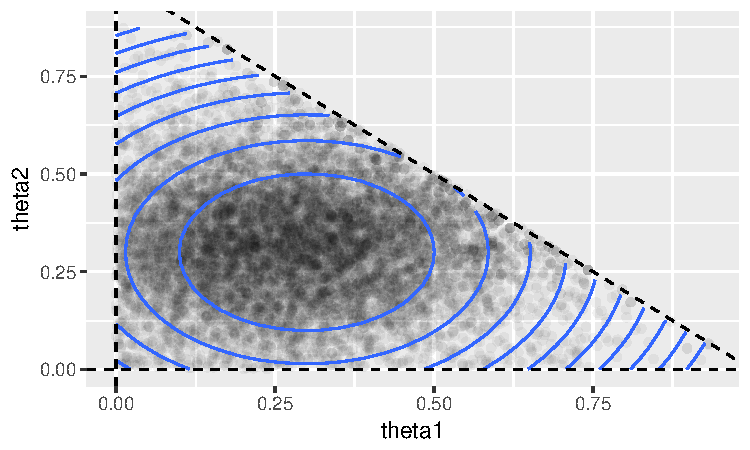
\includegraphics[width=1\textwidth]{linear_inequal_1}
    \caption{$n=10$ with true $\theta=[0.3,0.3]'$}
	\end{subfigure}
    \begin{subfigure}[b]{0.45\textwidth}
     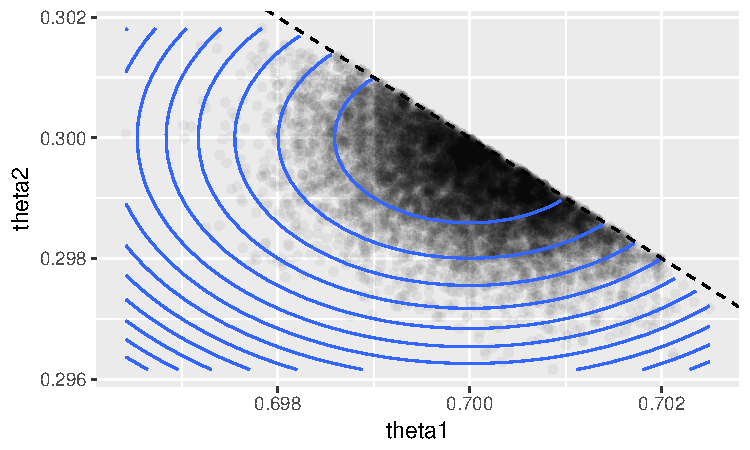
\includegraphics[width=1\textwidth]{linear_inequal_2}
     \caption{$n=10^4$ with true $\theta=[0.7,0.3]'$}
     	\end{subfigure}
\caption{Extrinsic posterior distribution of the normal mean $\theta$, with approximation to constraint $\theta_1+\theta_2\le 1$. Posterior is either loosely distributed near the center (panel (a)) or concentrated on the boundary (panel (b)) of the region. The extrinsic posterior has no samples outside of the region due to almost no relaxation.}
\label{linear_inequality}
\end{figure}

{\bf Example 3: Unit Circle}

Consider $\mc D$ as a two-dimensional unit cirlce $\{(\theta_1,\theta_2):\theta_1^2+\theta_2^2=1\}$, equivalently a $(2,1)$--Stiefel manifold. Within this space, $\eta(\theta;\mc D) =0 \forall \theta\in \mc D$ hence support expansion is necessary with moderate $\lambda$.

Let data $y_i\in \mathbb{R}^2$ for $i=1,\ldots,n$  be noisy realization from one point on unit circle:

$$y_i\sim \No(\theta, I_2\sigma^2),\text{ with } \theta'\theta=1,$$
where $\theta \in \mc D$ is assigned a von Mises--Fisher prior $\pi_{0,\mc D}(\theta) \propto \exp(F'\theta)$ (with corresponding unconstrained prior $\pi_{0,\mc R}(\theta) \propto \exp(F'\theta)\|\theta\|$).

 To generate data, we use $\theta= (\sqrt 3/2, 1/2)$, $\sigma^2=0.5^2$ and small $n=10$, in order to induce widely spread-out posterior $\theta$ on the manifold. We then use $F=(1,1)$ to induce a weakly informative prior for $\theta$ and an inverse-Gamma prior $\text{IG}(2,1)$ for $\sigma^2$. To assign extrinsic prior, we use $v(\theta)=|\theta'\theta -1|$ as the distance to circle and extrinsic prior $\tilde\pi_{0,\mc D}(\theta)= \exp(F'\theta) \exp(-\frac{|\theta'\theta -1|}{\lambda})$.

We test $\lambda = 10^{-3}$, $10^{-4}$ and $10^{-5}$ in three experiments, each corresponding to a different stability bound in leap-frog algorim. To visualize effects of stability bound, we restrict the maximum leap-frog steps $L$ to be $100$ and show how much space each setting can explore within one HMC iteration. Figure~\ref{unit_circle} plots its path of $L=100$ leap-frog steps.

Since the intrinsic posterior has closed-form $\pi_{\mc D}(\theta)\propto \exp [(F+\sum_i y_i/\sigma^2)'\theta]$, we collect the sample and compare the result. Each experiment is repeated $10$ times. Table~\ref{table_circle} shows the numeric 1-Wasserstein distance from its extrinsic approximate sample to exact posterior, and the posterior distance to $\mc D$, $v(\theta)$. All three settings have low approximation errors.

\begin{figure}[H]
\centering
   \begin{subfigure}[b]{0.8\textwidth}
    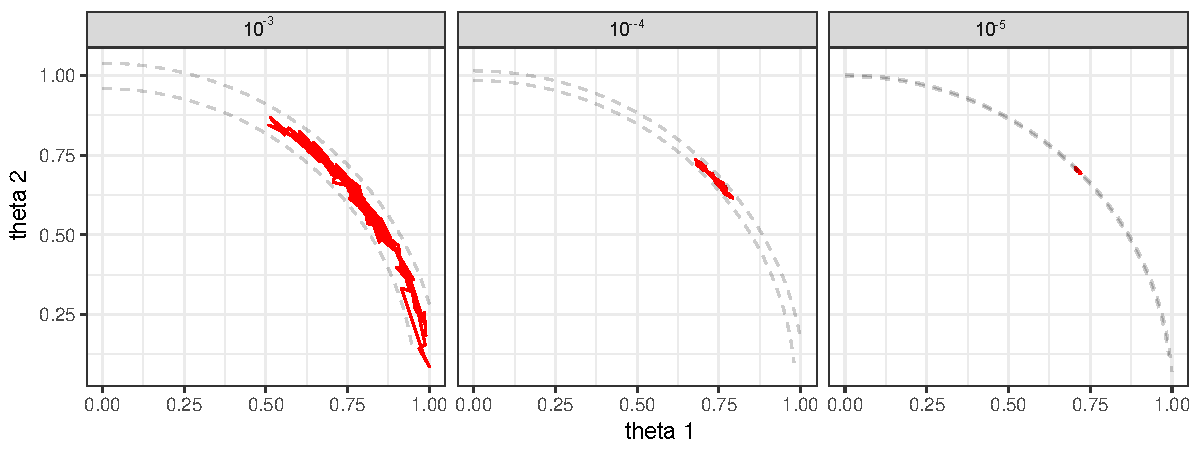
\includegraphics[width=1\textwidth]{unit_circle_100steps}
   % \caption{Path of 100 itegrator steps in one HMC iteraton}
	\end{subfigure}
    %\begin{subfigure}[b]{0.8\textwidth}
    % 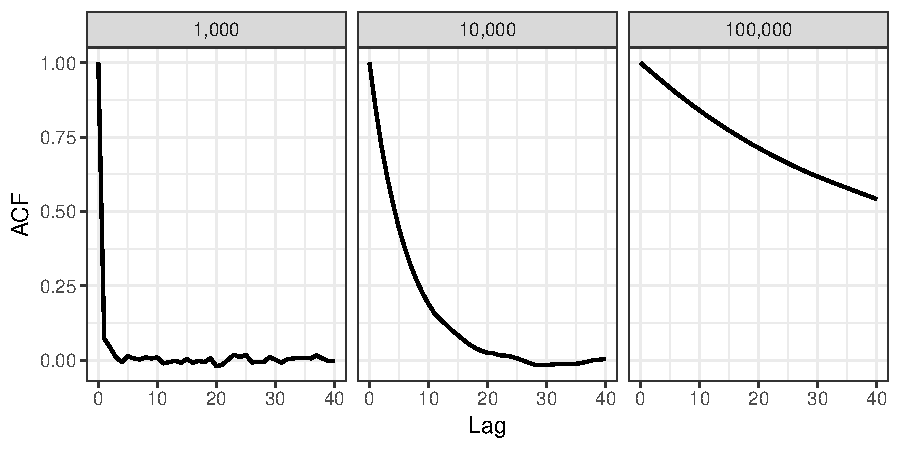
\includegraphics[width=1\textwidth]{unit_circle_acf}
    % \caption{Autocorrelation of $\theta_1$}
    % 	\end{subfigure}
    %\begin{subfigure}[b]{0.8\textwidth}
    %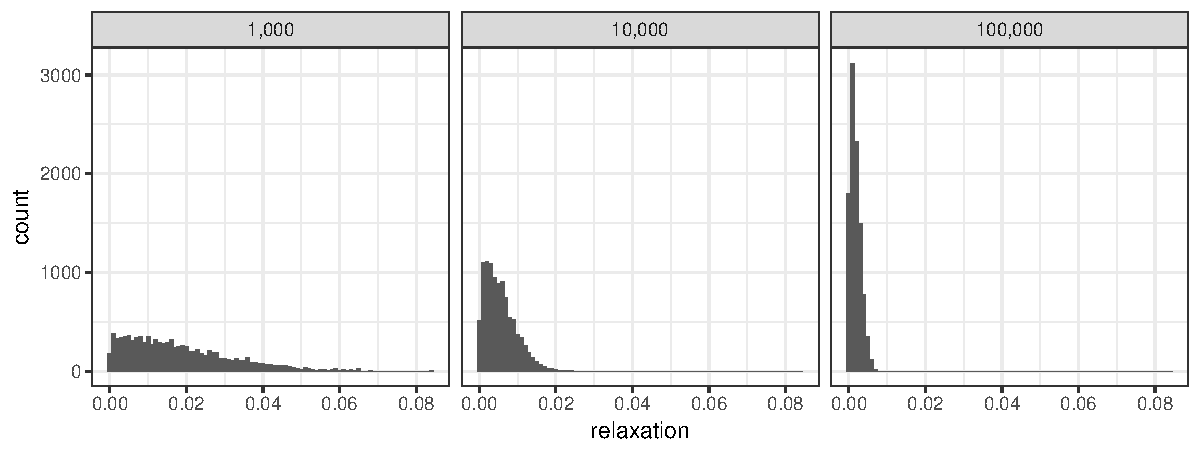
\includegraphics[width=1\textwidth]{unit_circle_violation}
    %     \caption{Posterior distribution of  $|\theta'\theta-1|$}
   % 	\end{subfigure}
\caption{Path of 100 itegrator steps in one HMC iteraton, sampling on a unit circle via extrinc prior with $\mc K(\theta)=\exp(-\frac{|\theta'\theta -1|}{\lambda})$, with $\lambda=10^{-4}$, $=10^{-5}$ and $=10^{-6}$. Larger relaxation in the narrowest direction of support (orthogonal vector to the circle) result in more efficient space exploration.}
\label{unit_circle}
\end{figure}

\begin{table}[H]
\centering
\small
\begin{tabular}{ c| c | c| c | c}
  \hline			
  $\lambda$  &  $10^{-3}$ & $10^{-4}$ & $10^{-5}$ & Exact  \\
  \hline
  \hline
  $W_1$ & 0.050 & 0.034  & 0.014   & 0.015 \\
  
   &  (0.019, 0.095) &(0.027, 0.037) &  (0.013,0.025)  & (0.0014,0.025)\\
  
  \hline
  $v(\theta) \mid y$ 
  & $9\times 10^{-4} $ 
  & $9\times 10^{-5} $ 
  & $9\times 10^{-6} $ \\
  & $(2.6 \cdot 10^{-5}, 3.3\cdot 10^{-3})$& $(2.0 \cdot 10^{-6}, 3.4\cdot 10^{-4})$& $(2.7 \cdot 10^{-7}, 3.5\cdot 10^{-5})$& 0\\
  \hline
  Avg. Time (sec/1000 eff. sample) & 4.6 & 15.3 & 40.5 &    \\
  \hline  
\end{tabular}
\caption{Average approximation error (with 95\% credible interval) of sampling from extrinsic distribution for 
a von--Mises Fisher distribution on a unit circle. The numeric 1-Wasserstein distance $W_1$ is low for all three settings and close to the numeric error in comparing two independent samples from the exact distribution; the posterior distance to $\mc D$, $v(\theta)= |\theta'\theta-1|$ is quite small.  The computing time needed for generating every $1000$ effective samples is shown. \label{table_circle}}
\end{table}

So far we have compared extrinsic approach with intrinsic one in settings with conjugate posterior. More advanced models often do not have simple form in constrained space. We now show two such examples where constrained models substantially outperform the unconstrained ones. Although these models create computing difficulty in intrinsic approach, they can be easily estimated extrinsically.


\subsection{Applications}

{\bf Example 3: Ordered Dirichlet Prior}

We first consider an ordered simplex in finite mixture model. The $(J-1)$--simplex is a vector $w=\{w_1,\ldots w_J\}$ with $1> w_1 \ge \ldots \ge w_J > 0$ and $\sum_{j=1}^J w_j=1$. This is built on the standard Dirichlet prior $Dir(\alpha)$, with $
\pi_{0, \mc D}(w) = \prod_{j=1}^J w_j^{\alpha-1} \1_{\sum_{j=1}^J w_j=1}$ with additional order constraint. In the base model Dirichlet prior,  index $j$ is exchangeable and its permutation does not change the likelihood. This leads to label-switching problem in mixture model estimation (reviewed in \cite{jasra2005markov}).

Imposing order constraint yields an ordered Dirichlet prior:

 \begin{equation}
\begin{aligned}
\label{ordered_dp_prior}
\pi_{0, \mc D}(w_1,\ldots w_J) \propto \prod_{j=1}^J w_j^{\alpha-1} \cdot \1_{\sum_{j=1}^J w_j=1} \cdot  \prod_{j=1}^{J-1}\1_{w_j \ge w_{j+1}}.
\end{aligned}
\end{equation}
where $w_j\in (0,1)$ for $j=1,\ldots,J$. Although the standard Gibbs sampling algorithm \citep{ishwaran2001gibbs} no longer applies in this setting, the ordered Dirichlet prior can be approximated by extrinsic prior:

 \begin{equation*}
\begin{aligned}
\tilde\pi_{0, \mc D}(w_1,\ldots w_J)  \propto \prod_{j=1}^J w_j^{\alpha-1} \cdot  \exp ( -  \frac{ \sum_{j=1}^J ( w_{j+1} - w_j )_+}{\lambda_1})
 \exp ( -  \frac{|{\sum_{j=1}^J w_j - 1}|}{\lambda_2})
\end{aligned}
\end{equation*}

We now adopt this simplex distribution in a normal mixture model with mixture means and common variance, for data $y_i\in \bb R^d$ indexed by $i=1,\ldots,n$:

\begin{equation*}
\begin{aligned}
y_i &\stackrel{indep}{\sim} \No(\mu_i,\Sigma),\qquad
\mu_i &\stackrel{iid}{\sim} G,\qquad
G(.) & = \sum_{j=1}^{J} w_j \delta_{\mu_j}(.),
\end{aligned}
\end{equation*}
where $\delta_{b}(a)=1$ if $a=b$ and $0$ otherwise.

We generate $n=100$ samples from $3$ components with true $\{w_1,w_2,w_3\}=\{0.6,0.3,0.1\}$ and two-dimensional means $\{\mu_1,\mu_2,\mu_3\} = \{[1,5], [3,3], [3,5]\}$ with identity covariance $\Sigma = I_2$. We assign weakly informative priors $\No(0,10 I_2)$ for each $\mu_j$ and inverse Gamma prior for the digonal element in $\Sigma=\diag(\sigma_1^2,\sigma_2^2)$ with $\sigma^2_1, \sigma^2_2\sim IG(2,1)$. We use $\lambda_1 = 10^{-6}$ to induce almost no relaxation on the ordering and $\lambda_2 = 10^{-3}$ on simplex constraint. To demonstrate the benefit of ordered Dirichlet, we compare the base model Dirichlet prior without order constraint, estimating via Gibbs sampling and HMC. 

Figure~\ref{dirichlet}(a) shows the contour of true posterior density of $\mu_j$'s. The small component sample size leads to large overlap among the posterior of $\mu_j$'s, generting in significant label-switching in both Gibbs and HMC under canonical Dirichlet prior. Figure~\ref{dirichlet}(b,c,d) show the traceplot of $w$. Ordered Dirchlet has almost no label-switching due to ordering.


\begin{figure}[H]
\begin{center}
   \begin{subfigure}[b]{0.3\textwidth}
    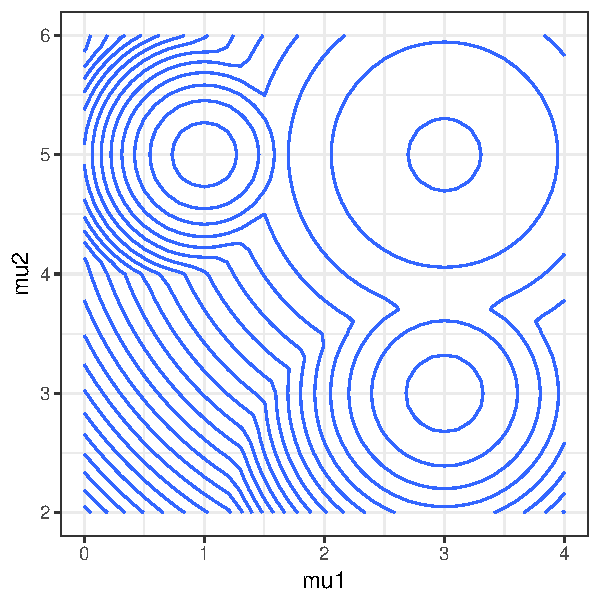
\includegraphics[width=1\textwidth]{fmm_mu_contour.pdf}
    \caption{Posterior density of the component means.}
    \end{subfigure}
    \end{center}
    \centering
   \begin{subfigure}[b]{0.32\textwidth}
    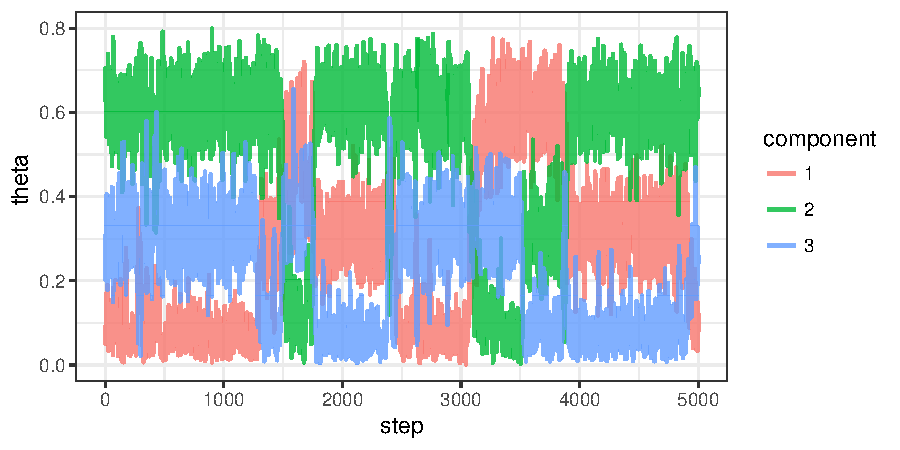
\includegraphics[width=1\textwidth]{fmm_w_gibbs.pdf}
    \caption{Gibbs sampling under canonical Dirichlet}
    \end{subfigure}
       \begin{subfigure}[b]{0.32\textwidth}
  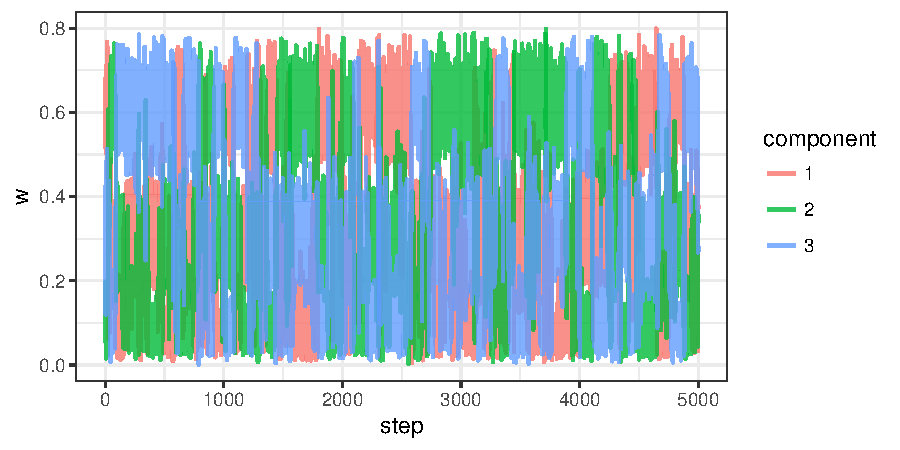
\includegraphics[width=1\textwidth]{fmm_w_hmc_unordered.pdf}
    \caption{HMC sampling under canonical Dirichlet, with extrinsic prior}
      \end{subfigure}
       \begin{subfigure}[b]{0.32\textwidth}
 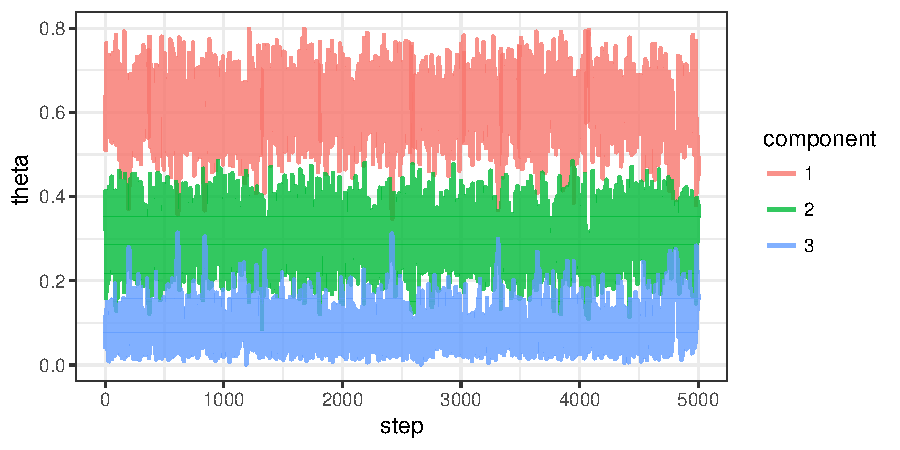
\includegraphics[width=1\textwidth]{fmm_w_hmc.pdf}
     \caption{HMC sampling under ordered Dirichlet, with extrinsic prior}
     \end{subfigure}
\caption{Contour of the posterior density of component means and traceplot of the posterior sample for the component weights $w$, in a 3-component normal mixture model. Panel (a) shows that there is significant overlap among component means $\mu_j$'s, creating label-switching issues in both Gibbs sampling (b) and HMC using canonical prior (c). The ordered Dirichlet prior significantly reducing label-switching (d).}
\label{dirichlet}
\end{figure}


{\bf Example 4: Orthonormal Low Rank Factorization of Multiple Undirected Networks}

We now consider a real data application in brain network analysis. The brain connectivity structures are obtained in the data set KKI-42 (Landman et al. 2011), which consists of $21$ healthy subjects without any history of neurological disease. Each subject has two brain network observations from scan--rescan, yielding a total of n = 42. Each observation is a $V\times V$ symmetric network $A_i$, recorded as adjacency matrix $A_i$ for $i=1,\ldots,n$. For the $i$th matrix $A_i$, $A_{i,k,l} \in \{0,1\}$ is the element on the $k$th row and $l$th column of $A_i$, with $A_{i,k,l}=1$ indicating there is an connection betwen $k$th and $l$th region, $A_{i,k,l}=0$ if there is no connection. The regions are constructed via the Desikan et al. (2006) atlas, for a total of V = 68 nodes.

The ambient dimension of observation is $V(V-1)/2=2,278$, which is significantly larger than sample size $n=40$. They potentially contain observational error in recording connectivity, and the  diagonal in each $A_{i}$ is missing due to the lack of self-connectivity. These facts motivate a Bayesian low-rank approach. We consider a symmetric tensor decomposition model:

\begin{equation*}
\begin{aligned}
& A_{i,k,l} \sim \text{Bern}( \frac{1}{1+ \exp(-\psi_{i,k,l}- Z_{k,l})})\\
& \psi_{i,k,l} = \sum_{r_1=1}^{d_1}\sum_{r_2=1}^{d_2} D_{r_1,r_2} W_{i,r_2} U_{k,r_1} U_{l,r_1}  \\
\end{aligned}
\end{equation*}
for $k>l$, $k=2,\ldots, V$, $i=1,\ldots,n$; $U$ is $V\times d_1$ matrix, $W$ is $n\times d_2$ matrix; $D$ is a $d_1\times d_2$ array. The  $V\times V$ matrix $Z$ is almost unstructural except symmetric $Z_{k,l}=Z_{l,k}$, which is commonly used to induce low-rank in the decomposition \citep{durante2016nonparametric}.


This model is a special Tucker decomposition with a sparse core tensor, whose diagonal plane is equal to $D$ and $0$ for other elements. The Tucker decomposition is more flexible than another routinely used decomposition, namely parallel factor analysis (PARAFAC). The PARAFAC assumes all ranks are equal and the core tensor $D$ only has non-zero value when all its sub-indices are equal. In this case, PARAFAC would assume $d_1=d_2$. The additional flexibility in the Tucker is appealing, as one could utilize the varying rank over different sub-direction (mode) of the tensor. On the other hand, a completely unconstrained Tucker decomposition is not identifiable in the matrices and core tensor, due scaling. For example, one can multiply a $d_1\times d_1$ non-zero diagonal matrix $R$, to $U$ and obtain $U^*=UR$ obtain $D^{*}_{.,r_2,.}=R^{-1}D_{.,r_2,.}R^{-1}$ for $r_2=1,\ldots,d_2$. This leaves the likelihood unchanged, creating identifiability issue. 

Therefore, we consider applying some constraint on the Tucker decomposition. Motivated by high-order singular value decomposition, we impose orthonormality constraints $U'U=I_{d_1}$ and $W'W=I_{d_2}$. \cite{hoff2016equivariant} previously obtained conjugated posterior for Tucker decomposition under orthonormality constraint, however, the symmetry in undirectedness of networks breaks the conjugacy.

We assign normal prior for $U_{k,r_2}\sim \No(0,\phi_{1})$, $W_{i,r_1}\sim \No(0,\phi_2)$, $Z_{k,l}\sim \No(0,\phi_3)$, $D_{r_1,r_2}\sim No(0, \phi_{4,r_1,r_2})$ for all $i,k,l,r_1,r_2$, and inverse-Gamma prior $\phi_1,\phi_2,\phi_3\stackrel{indep}{\sim} \text{IG}(2,1)$, $\phi_{4,r_1,r_2}= \tau_{r_1}\tau_{r_2}$, with $\tau_{r_1},\tau_{r_2}\stackrel{indep}{\sim} \text{IG}(2,1)$ for all $r_1,r_2$. We

%we assign multiplicative inverse gamma distribution \citep{bhattacharya2011sparse} $\phi_{4,r_1,r_2}= \prod_{m_1=1}^{r_1} \nu_{1,m_1} \prod_{m_2=1}^{r_2}  \nu_{2,m_2}$ with $\nu_{1,1},\nu_{2,1} \stackrel{indep}{\sim} \text{IG}(a_1,1)$ and $\nu_{1,m},\nu_{2,m}\stackrel{indep}{\sim} \text{IG}(a_2,1)$ for $m\ge 2$. This induces increasing concentration toward zero as $r_1,r_2$ increase, allowing adaptive choosing of latent dimensions. We set $a_1=a_2=5$ in this application.

To allow estimation for model with orthonormality constraint, we use extrinsic prior with $\mc K(\theta) = \exp( - \frac{(U'U-I_{d_1})^2 + (W'W-I_{d_2})^2  }{\lambda})$ and set $\lambda=10^{-3}$. To compare, we also test with the same model configuration without the orthonormality constraint. We run both models for $10,000$ steps and discard the first $5,000$ steps. Figure~\ref{tucker} plots the traceplot and autocorrelation for matrix $U$. Unconstrained base model has severe convergence issue due to the non-identifiability, while constrained model converges and show low autocorrelation for all the parameters.

\begin{figure}[H]
   \begin{subfigure}[b]{1\textwidth}
    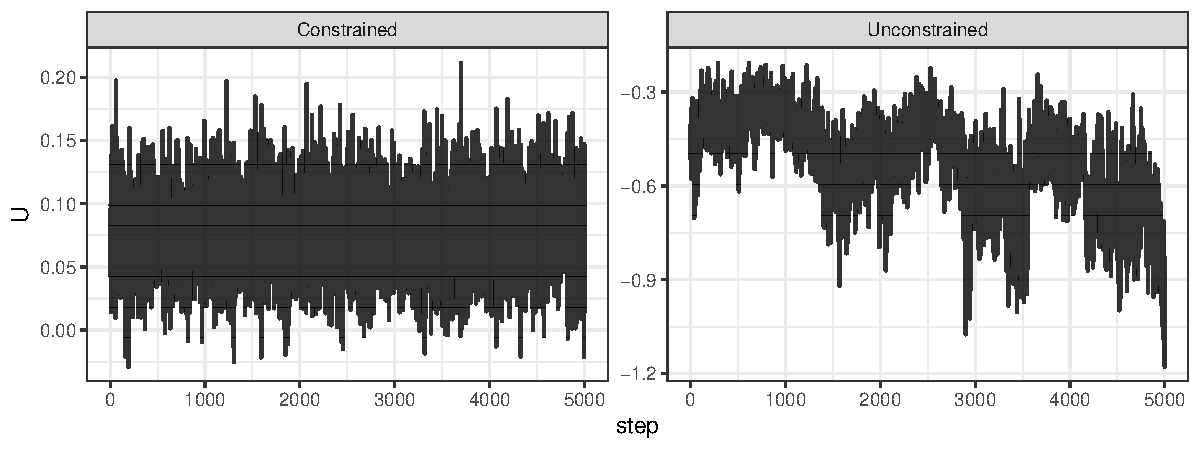
\includegraphics[width=1\textwidth]{tucker_traceplot.pdf}
    \caption{Traceplot of $U_{1,1}$.}
    \end{subfigure}
    \begin{subfigure}[b]{1\textwidth}
    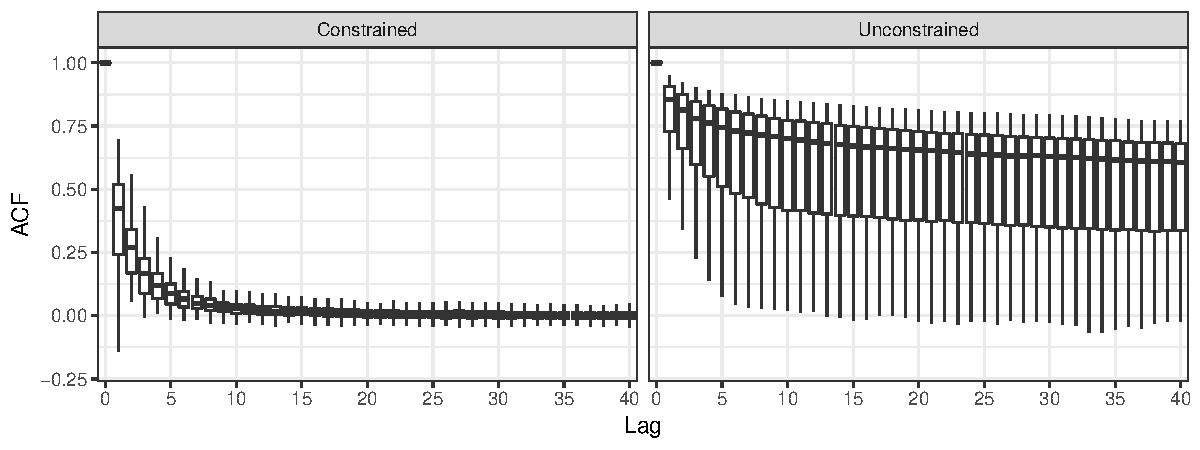
\includegraphics[width=1\textwidth]{tucker_acf.pdf}
    \caption{ACF of all elements in $U$}
    \end{subfigure}
\caption{Orthonormality constraint in the tensor decomposition modelallows convergence and rapid mixing on the factor matrix (left column); whereas unconstrained model does not converge due to free scaling. Traceplot for one parameter in factor matrix $U$ and boxplot for autocorrelations of all parameters are shown.}
\label{tucker}
\end{figure}

\section{Discussion}

The estimation difficulty associated with parameter constraint often hinders the development of new models. Often one needed to carefully avoid models without conjugate posteriors, or skillfully re-parameterize the model for a more tractable algorithm. The extrinsic approach we introduced significantly reduces the burden. Through space expansion, it allows conventional toolbox such as HMC to be easily adopted to sample posterior without closed-forms. This allows researchers to impose constraints more freely in modeling and simplifies the way to incorporate constraint information about the functional of parameters.

We show the approximation error of the extrinsic approach can controlled via tuning parameter, with some trade-off between computing time and accuracy. A potentially more efficient strategy would be obtaining a rough approximate first in $\mc R$, then projecting into $\mc D$. \cite{lin2016extrinsic} developed algorithms similar to this idea and obtained consistency result for point estimation. A useful task would be to find an optimal projection also quantifying the uncertainty associated with finite sample. Lastly, the normalization of parameters over constrained space can sometime yield intractable integral, known as `doubly stochastic' problem. We expect that the proposed extrinsic prior can be adapted and used together with the various existing solutions \citep{rao2016data,stoehr2017noisy}.



\bibliography{reference}
\bibliographystyle{chicago}

\section{Appendix}

Remark 1 proof:
\begin{proof}[Proof]
Let $g:\mathbb{R}^p\rightarrow \mathbb{R}$ be a 1-Lipschitz continuous function, i.e. $\|g(x)-g(y)\|\le \|x-y\|$, denoted by $\|g\|_L\le 1$. 
By Kantorovich-Rubinstein duality, the 1-Wasserstein distance based on Euclidean metric equals to: 

\begin{equation}
W_1(\Pi,\tilde\Pi)=\underset{g:\|g\|_L\le 1}\sup \int g(x) \Pi(dx) -  \int g(y) \tilde\Pi(dy) 
\end{equation}

Taking $g(\theta)=\exp(-\lambda^{-1}v(\theta))$ yields
	\begin{equation}
	\begin{aligned}
	m_\lambda
	& = \int_\mathbb{R}  \left[ \int_{v^{-1}(x)} \frac{ \exp(- \lambda^{-1} v(\theta) ) \pi_{\mc R}(\theta)}{ J v(\theta) } \mathcal{H}^{p-d}(d \theta) \right] \mathbbm{1}_{x \ge 0}  d x \\
	& = \int_\mathbb{R}  m(x)\exp(- \lambda^{-1} x ) \mathbbm{1}_{x \ge 0}  d x .
		\end{aligned}
	\end{equation}
	
Taking $g(\theta)={\mathbbm{1}_{v(\theta)=0}}$ yields 
	\begin{equation}
	m_0
	= \int_\mathbb{R} \left[ \int_{v^{-1}(y)} \frac{ \pi_{\mc R}(\theta) }{ J v(\theta) } \mathcal{H}^{p-d}(d \theta) \right]\mathbbm{1}_{y=0} dy   =  \int_{v^{-1}(0)} \frac{ \pi_{\mc R}(\theta) }{ J v(\theta) } \mathcal{H}^{p-d}(d \theta) =m(0)
	\end{equation}
	
	Clearly $m_\lambda \ge m_0$.
	
1. Asymptotic result:
	
We have
	
	\begin{equation}		
	\label{wass0}
		\begin{aligned}
	&\underset{g:\|g\|_L\le 1}\sup\int g(\theta)  \left[ \frac{ \exp(- \lambda^{-1} v(\theta)) } {  m_\lambda}  - 
	 \frac{ \mathbbm{1}_{v(\theta)=0} } {  m_0} 
	\right]  \frac{\pi_{\mc R}(\theta)}{Jv(\theta)} \mc H^{p-d}(d \theta) \\
	&= \underset{g:\|g\|_L\le 1}\sup\int_\mathbb{R}  \mathbb{E}(g(\theta) \mid x)  \left[ \frac{ \exp(- \lambda^{-1} x) \mathbbm{1}_{x \ge 0}} {  m_\lambda}  - 
	 \frac{ \mathbbm{1}_{x=0} } {  m_0} 
	\right] d x \\
		&=	\underset{g:\|g\|_L\le 1}\sup\int_\mathbb{R}  \mathbb{E}(g(\theta) \mid x)  \left[ \frac{  1} {  m_\lambda}  - 
	 \frac{ 1 } {  m_0} 
	\right]\mathbbm{1}_{x=0} d x  + \underset{g:\|g\|_L\le 1}\sup\int_\mathbb{R}  \mathbb{E}(g(\theta) \mid x)\frac{ \exp(- \lambda^{-1} x)} {  m_\lambda}  
	  \mathbbm{1}_{x > 0} d x \\
	& \le \underset{g:\|g\|_L\le 1}\sup \|\mathbb{E}(g(\theta) \mid 0)\| \left[ \frac{ 1 } {  m_0} -\frac{  1} {  m_\lambda}   
	 \right] + \frac{1} {  m_0} \underset{g:\|g\|_L\le 1}\sup \int_\mathbb{R}  \|\mathbb{E}(g(\theta) \mid x)\| { \exp(- \lambda^{-1} x)}
	\mathbbm{1}_{x > 0} d x \\	
	  \end{aligned}
	  \end{equation}
	  
	 	  
	Note $m_\lambda\le \int_\mathbb{R} m(x) \mathbbm{1}_{x \ge 0}  dx =\int_\mathbb{R} \pi_{\mc R}(\theta) =1$. By dominated convergence theorem, 

\begin{equation}
	\lim_{\lambda\rightarrow 0}m_\lambda= \int_\mathbb{R}  m(x) \lim_{\lambda\rightarrow 0}\exp(- \lambda^{-1} x ) \mathbbm{1}_{x \ge 0}  d x = m_0.
\end{equation}

	
	   Since 
	  $ \underset{g:\|g\|_L\le 1}\sup \int_\mathbb{R}  \|\mathbb{E}(g(\theta) \mid x)\| { \exp(- \lambda^{-1} x)} dx \le \int_\mathbb{R} \underset{g:\|g\|_L\le 1}\sup \|\mathbb{E}(g(\theta) \mid x)\| { \exp(- \lambda^{-1} x)} dx$,
	  letting $q_\lambda=	  \underset{g:\|g\|_L\le 1}\sup \|\mathbb{E}(g(\theta) \mid x)\| { \exp(- \lambda^{-1} x)}
	\mathbbm{1}_{x > 0}  $, we have $0\le q_1-q_{\lambda_1}\le q_1-q_{\lambda_2}$ for $1\ge\lambda_1\ge \lambda_2$, by monotone convergence theorem, $\lim_{\lambda\rightarrow 0}\int [ q_1(x)-q_\lambda(x)]dx = \int [q_1(x)- q_0(x) ]dx$ hence $\lim_{\lambda\rightarrow 0}\int q_\lambda(x)dx =0$. Combining the results yields 
	  
	  
	
	\begin{equation}
 \underset{\lambda \rightarrow 0}\lim W_1(\Pi,\tilde\Pi)=0.	  \end{equation}
	  
	  2. Non-asympotic result:
	

	\begin{equation}
	\label{wass1}
	\begin{aligned}
	\frac{1}{m_0}-\frac{1}{m_\lambda} & \le  \frac{   \int_\mathbb{R}  m(x) \exp(- \lambda^{-1} x ) \mathbbm{1}_{x > 0}  d x } {  m_0^2}  \\
	&= \frac{1}{ m_0^2} \left[ \int_0^{t}  m(x) \exp(- \lambda^{-1} x ) dx + \int_t^{\infty}  m(x) \exp(- \lambda^{-1} x ) dx \right] \\
	&\le \frac{1}{ m_0^2} \left[  \underset{t^*\in (0,t)}\sup m(t^{*})\int_0^{t} \exp(- \lambda^{-1} x ) dx + \exp(- \lambda^{-1} t )\int_t^{\infty}  m(x) dx  \right] \\
	&\le \frac{1}{ m_0^2} \left[\lambda \underset{t^*\in (0,t)}\sup  m(t^{*})  + \exp(- \lambda^{-1} t ) \right] 
	\end{aligned}
\end{equation}

	\begin{equation}
		\label{wass2}
	\begin{aligned}
	 & \underset{g:\|g\|_L\le 1}\sup\int_\mathbb{R}  \|\mathbb{E}(g(\theta) \mid x)\| { \exp(- \lambda^{-1} x)}	\mathbbm{1}_{x > 0} d x \\
	&\le \underset{g:\|g\|_L\le 1}\sup\underset{t^*\in (0,t)}\sup \|\mathbb{E}(g(\theta) \mid t^*)\|	
	\int_0^{t} \exp(- \lambda^{-1} x ) dx + \exp(- \lambda^{-1} t ) \underset{g:\|g\|_L\le 1}\sup \int_t^{\infty}   \|\mathbb{E}( g(\theta )\mid x)\| dx \\
&\le \underset{g:\|g\|_L\le 1}\sup\underset{t^*\in (0,t)}\sup \|\mathbb{E}(g(\theta) \mid t^*)\|	\lambda + \exp(- \lambda^{-1} t ) \underset{g:\|g\|_L\le 1} \sup \mathbb{E}(\| g(\theta )\|) \\
	\end{aligned}
\end{equation}

Combining \eqref{wass0}\eqref{wass1}\eqref{wass2}, $k_1=\underset{g:\|g\|_L\le 1}\sup\underset{t^*\in [0,t)}\sup \|\mathbb{E}(g(\theta) \mid t^*)\|$, $k_2=\underset{g:\|g\|_L\le 1} \sup \mathbb{E}(\| g(\theta )\|)$, $k_3= \underset{t^*\in (0,t)}\sup  m(t^{*})$


\begin{equation}
\begin{aligned}
& \underset{g:\|g\|_L\le 1}\sup \int g(x) \Pi(dx) -  \int g(x) \tilde\Pi(dx) \\
	%&\le  \frac{k_1}{ m_0^2} \left[\lambda k_3  + \exp(- \lambda^{-1} t ) \right] 
	%+ \frac{1} {  m_0} [ k_1	\lambda + \exp(- \lambda^{-1} t )k_2 ]\\	
	& \le \lambda (\frac{k_1 k_3}{m_0^2} + \frac{k_1}{m_0}) + \exp(- \lambda^{-1} t )(\frac{k_1}{m_0^2} + \frac{k_2}{m_0})
\end{aligned}
\end{equation}


\end{proof}
\end{document}
